\chapter{EVOLUTION OF TECHNOLOGY}\label{chp:Evaluation of Technology}

This chapter provides an overview of artificial intelligence, machine learning, and image processing. 

\section{ARTIFICIAL INTELLIGENCE}

Artificial intelligence (AI) is the ability of a computer to perform various activities similar to an intelligent entity. In order to understand whether these various activities are carried out by artificial intelligence, humans need observation. There are two different alternatives to observing intelligence. The first is introspection through the observation of thoughts, and the second is the observation of behavior, which is the result of intelligence activities.

In the 1930s, Alan Turing, a pioneer mathematician, took part in the construction of the first electronic computer. In 1950, he proposed the "Turing Test" to answer whether machines can think, which is shown in Figure \ref{fig:TuringTest}.

\begin{figure}[htbp]
\centering
\fbox{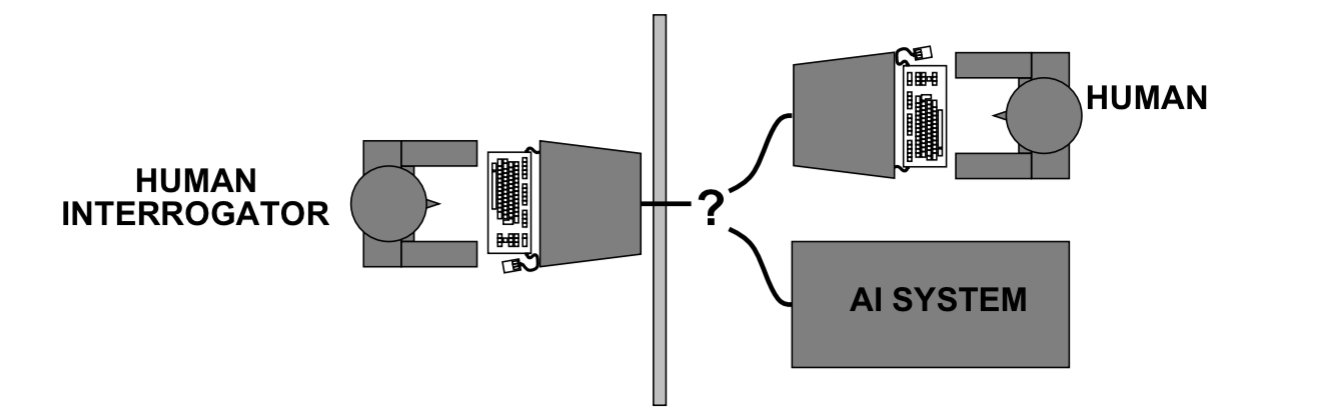
\includegraphics[width=.8\columnwidth]{figures/TuringTest.png}}
\caption{Turing test \cite{russel2010}}
\label{fig:TuringTest}
\end{figure}

In the Turing Test \cite{turing2009computing}, the subject communicates with the interrogator via a terminal. If the interrogator does not understand whether the subject is human or a machine, the subject is considered to have passed the Turing Test.

In the following years, programs such as SHRDLU \cite{winograd1972understanding}, and ELIZA \cite{mauldin1994chatterbots} were successful in the Turing Test even though they do not fully represent human intelligence. For example, the ELIZA program asks questions or forms sentences in response to the answers received from the user. Like a therapist, ELIZA asks open-ended questions. In addition, ELIZA forms the questions according to the predefined words in the answer. Hence, when there is an input sentence that contains the word "friend,'' it would reply with "Tell me about your friend.". Thus, there is no understanding or representation of human intelligence. Therefore, based on statistical information, it is possible to pass the Turing Test.

On the other hand, John Searle, who argued that machines could never have the ability to think and understand, proposed the Chinese Room Experiment \cite{preston2002views}. In the Chinese Room Experiment, a person in the locked room does not speak Chinese. An instruction manual tells what to do if specified Chinese letters have come to the room. The person who is in the room writes in Chinese using this guide. For an outside observer, there is a person who understands Chinese in the room. Understanding Chinese is not replacing symbols with certain symbols. In this respect, he suggests that computer programs will never have the ability to understand.

There are three types of AI and; they are grouped based on their abilities. Weak AI (Narrow AI) \cite{confbringsjord2003artificial} is the performing intelligent actions on a specific field (Narrow-Area) like the ability to drive a car. It is mainly emulating intelligence. General intelligence (Strong AI) \cite{confbringsjord2003artificial} is the ability to perform human-like intelligence in various tasks. It has equivalent human behavior. Lastly, Super Intelligence \cite{bostrom2003ethical} is the performing intelligent action that exceeds humans' performance in all domains.

Apart from this, there are many areas of AI such as Knowledge-based systems \cite{davis1982knowledge}, Natural Language Processing \cite{dale2000handbook}, Fuzzy Logic \cite{zadeh1996fuzzy}, Robotics \cite{brady1984artificial}. 

After a brief introduction to artificial intelligence, the following subsection will make an introduction to machine learning and machine learning types.

\section{MACHINE LEARNING}
Machine learning is the ability of machines to learn from experiences, make decisions regarding similar situations in the future, and produce solutions to problems \cite{booksmichie1994machine}. Therefore, machine learning makes generalizations for a new related event by searching previous cases and outcomes \cite{booksmichie1994machine}.

There are three types of learning methods: Supervised, Unsupervised, and Reinforcement (Figure \ref{fig:MachineLearningTypes}). The first one, Supervised Learning, requires an external intervention or an internal mechanism to achieve the desired output values. The secondary, Unsupervised Learning, utilizes  the analysis of the inputs without external intervention. Last but not least, Reinforced Learning, acquires knowledge by interacting with its surrounding environment and processing the data via a trial and failure approach \cite{sathya2013comparison}.

\begin{figure}[htbp]
\centering
\fbox{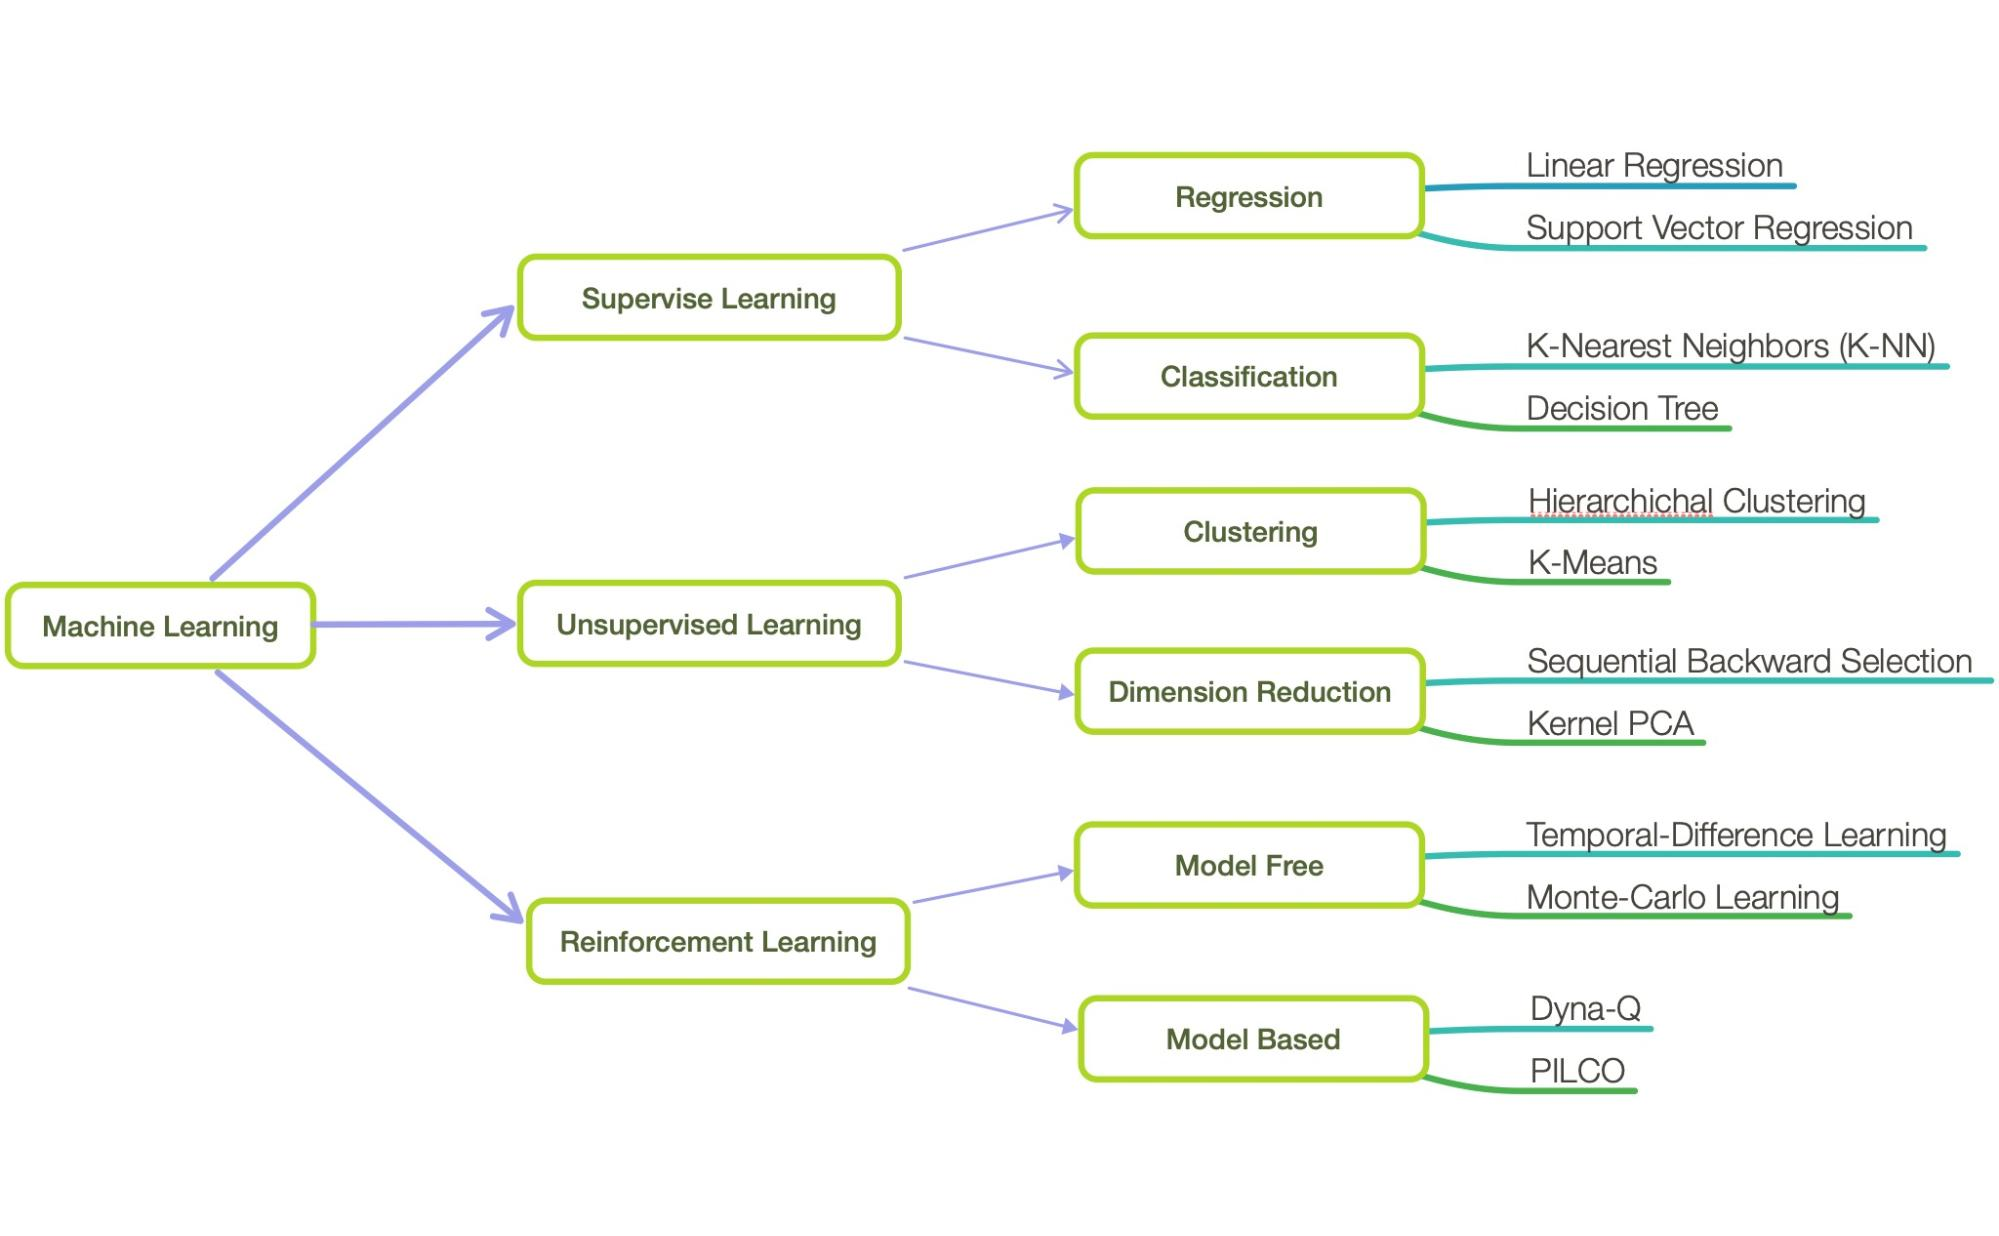
\includegraphics[width=.8\columnwidth]{figures/MachineLearningTypes.jpg}}
\caption{Machine learning types}
\label{fig:MachineLearningTypes}
\end{figure}

\subsection{SUPERVISED LEARNING}

In supervised learning, both the input and output values are feeded to the algorithm in the learning phase. Therefore in the learning stage, the application processes input values and compares the desired output values with the result of the application. The difference between expected and output is treated as an error. The error value is calculated by the performance function. Result of the performance function is returned to the system to minimize this error. As a result, this process continues until the error is minimized.

In this error minimization, the algorithm generalizes outputs based on provided input data (i.e. Test Set) which is also called a supervised learning algorithm. This process could result in four main problems. We will go through each of these problems. 

The first one is the Bias-Variance trade-off \cite{geman1992neural} (Figure \ref{fig:BiasAndVariance}). A supervised learning algorithm has a high variance in predicting results with a significant deviation from the mean and other predictions when training in various practice collections. Therefore, the variance measures the contiguity of the data predicted by the model to the actual data. On the other hand, supervised learning algorithms are highly biased if inaccurate when forecasting the output for different training sets. Therefore, the bias measures how incorrect the model is. As a result, the success of the algorithm is usually associated with the amount of bias and variance \cite{james2003variance}. In most cases, the compromise between bias and variance is inevitable. In most of the algorithms, this trade-off can be modified with a parameter or automatically. 

\begin{figure}[htbp]
\centering
\fbox{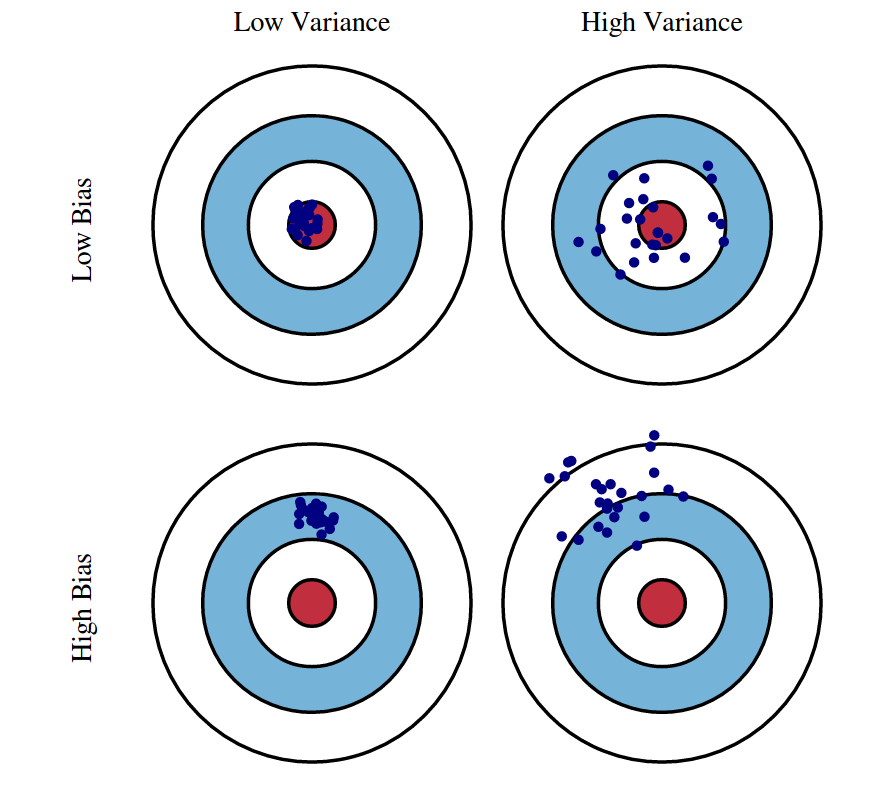
\includegraphics[width=.6\columnwidth]{figures/BiasAndVariance.png}}
\caption{Graphical illustration of bias and variance \cite{biasandvarianceillustration}}
\label{fig:BiasAndVariance}
\end{figure}

The second problem is the complexity of the problem and the amount of training data. The amount of data required to train an algorithm depends on the complexity of the problem. In relatively simple problems, the small set of training data will be enough to achieve learning. However, complex problems, which require feature extraction in multiple dimensions, need a well-distributed and an extensive training set.

The third problem is the number of dimensions in an input space. The larger the number of dimensions, the more difficult the algorithm will be to learn because of the high variance, as redundant dimensions hide features. For this problem, there are algorithms to reduce dimensions like autoencoders. Another approach for this problem would be manually extracting features before feeding them to the algorithm. Another strategy would be fine-tuning the supervised learning algorithm to low variance, and high bias may also solve the problem.

Apart from this, there is a possibility of overfitting in complex problems even if there is no noise. This type of overfitting is related to algorithms being unable to model the training data, also called deterministic noise. There are a few possible solutions to this problem. The first possible solution is removing data which caused overfitting from the data set by hand. Another approach is to use other algorithms to remove data that caused overfitting from possible errors from data sets. Another strategy would be to use early stopping to prevent overfitting. For example, the drop-out layer is used in deep neural networks to prevent overfitting.

Supervised learning is used to tackle two types of problems: Regression and Classification. Regression is a collection of statistical techniques to predict the associations between variables. It tries to model and analyze multiple variables when concentrating on the connection between a dependent variable and one or more unrelated elements. Moreover, regression is used extensively for prediction and projection.

There are two types of regression - namely, parametric and non-parametric. In parametric regression, the number of dimensions is predefined, such as Linear Regression and Ordinary Least Squares. On the other hand, non-parametric regression has no defined dimensions. As a result, regression models are often helpful in prediction, even if the assumptions are moderately wrong. Nevertheless, in many cases, regression models can not operate optimally. In the following paragraphs, we will examine a few Regression algorithms.

The linear regression method is a statistical technique that establishes a linear relationship between the independent variable and the dependent variable to estimate the feature variable \cite{tan2016introduction}. In a linear regression equation, where an example is shown in equation \ref{linear_regression_equation}, \(x\) represents estimator for a problem, \(y\) is the response variable a the slope of the regression line is \(a_1\) and, \(b_1\) is the point at which the regression line intersects the ordinate axis.

\begin{equation} \label{linear_regression_equation}
y = a_1x + b_1x
\end{equation}

The main working principle of the support vector machine (SVM) is to divide the data into the broadest categories that separate them from each other, which is based on Vapnik–Chervonenkis theory developed by Vladimir Vapnik and Alexey Chervonenkis. SVM is successfully used in applications such as pattern recognition, time series analysis, and classification. SVM can be applied to both linear and non-linear data. The regression process is carried to the high dimensional feature spaces by the kernel function in non-linear data.

The other type in which supervised learning is used is a classification that assigns each input vector to a finite number of discrete categories \cite{harrington2012machine}. One of the most known examples of this classification is classifying emails as spam or not. Beside that, machine learning studies for classification are used in various fields such as stock estimation, customer risk analysis for bank credit, earthquake prediction, text classification, disease diagnosis, genetic studies. In the following paragraphs, few classification algorithms were examined.

K-Nearest Neighbor Algorithm (K-NN) is a memory-based classification, where its popular use is in the data mining domain. In K-NN, after the classes of the sample set are determined, the method determines which new observation belongs to which class. Here, the samples are considered a point in n-dimensional space, and the parameter k, the number of neighbors closest to the given point, is determined \cite{cover1967nearest}. The distances of all other points to the given point are calculated individually because of this method based on distance calculation. 

\begin{equation} \label{euclidean_distance_equation}
d(x,y) = \sqrt{\sum_{j=1}^{N}(x_j - y_j)^2}
\end{equation}

The Euclidean Distance shown in equation \ref{euclidean_distance_equation} is commonly used to calculate the distance between observations. The smallest k is selected according to the distance values calculated here \cite{hall2008choice}.

\begin{figure}[htbp]
\centering
\fbox{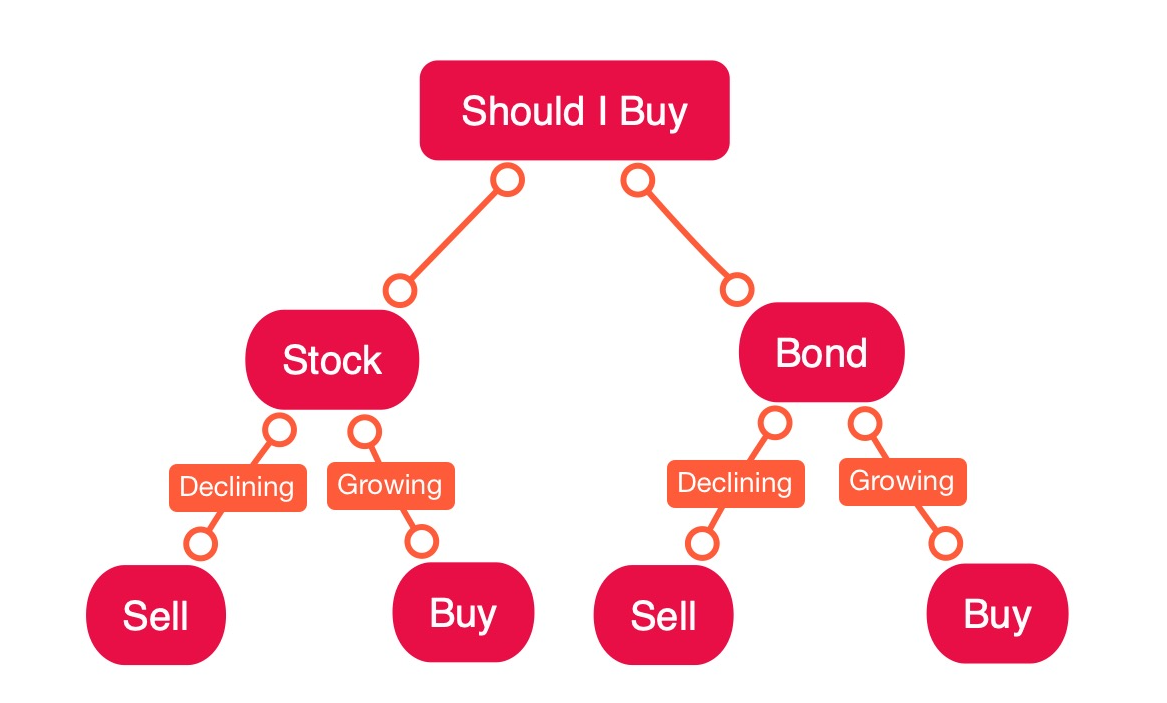
\includegraphics[width=.6\columnwidth]{figures/DecisionTree.png}}
\caption{Decision tree}
\label{fig:DecisionTreeExample}
\end{figure}

Another classification algorithm is decision trees. They consist of internal decision nodes and end leaves (Figure \ref{fig:DecisionTreeExample}). A decision tree tries to establish which class the data with a particular class will be included in, starting from the node with the highest information gain \cite{hssina2014comparative}. One of the most commonly used algorithm to create a decision tree in data mining is the ID3. The main principle of the ID3 algorithm is to classify objects by testing the values of their attributes \cite{jin2009improved}.

\subsection{UNSUPERVISED LEARNING}

The purpose of unsupervised learning is to model the underlying structure or distribution of the data to extract information from raw data. Unlike Supervised Learning, there is no data to guide the learning process. It is generally used for clustering, finding relationships between attributes and size reduction. Besides, the results obtained with the unsupervised learning algorithm can be used for supervised learning \cite{chao2011machine}.

A critical point for unsupervised learning is that, while the information transmitted to learning algorithms is highly rich in underlying composition, the objectives and prizes for training are usually very narrow. Therefore, in this type of objective and prize, the algorithm should understand the information instead of applying it to a specific task. As a result, using unsupervised learning as a sub-task might improve the results even in supervised learning tasks (e.g., Deep Learning Tasks).

Unsupervised learning is used for clustering and dimension reduction. Clustering is a data grouping with similar characteristics in a data set. Therefore, there are high similarities within the same cluster, and there are low similarities between clusters. K-Means and Hierarchical Clustering are some of the commonly used clustering algorithms. These algorithms are frequently used in areas such as customer segmentation, market segmentation, and computer vision.

Clustering is a very fundamental task to discover unknown elements of unlabeled data. However, success measures depend on the users' demands, such as a minimum number of clusters. On the other hand, understanding the underlying knowledge in the cluster solely depends on the user. In the following paragraphs, we are examining K-Means and Hierarchical Clustering algorithms.

Hierarchical clustering (Hierarchical Cluster Analysis - HCA) is a cluster analysis technique designed to produce a cluster hierarchy. There are two types of HCA; namely  Agglomerative (Bottom-Up) and Divisive (Top-Down). Agglomerative type starts by turning each data into a cluster, and then the clusters that are close to each other in distance form a new cluster. Divisive is the opposite of Agglomerative. At first, all data is created in a single set, then this cluster is fragmented and reclustered. 

After the K value (the number of clusters) is determined by the user in K-Means, the algorithm selects random K points in the data set. Then, it calculates the distance between each point and random k-points to assign the data to a cluster. After assigning the points to clusters, k points are re-calculated based on the data in each cluster. Finally, the same distance calculation is performed according to the new k points. The method continues until a point is not assigned to relevant groups.

Real-life data has a large number of dimensions. This size of data brings complexity. This complexity also creates some problems; for example, there would be a significant increase in the amount of time and resources required to build a model. In addition, there is a high correlation between some attributes, leading to overfitting \cite{sonawale2015dimensionality}. Dimensionality reduction, which decreases unrelated features or merges attributes into smaller sets of dimensions \cite{biricik2012comparing}, helps us solve this problem. The following paragraphs examine the Kernel Principal Component Analysis (KPCA) and Sequential Feature Selection (SFS). 

KPCA is based on standard deviation, covariance, eigenvectors, and eigenvalues. The use of integral operator kernel functions and non-linear maps can correctly compute main parts in high-dimensional feature spaces associated with input space \cite{scholkopf1997kernel}.

SFA uses a greedy approach which is very useful for computationally complex problems. However, it might produce unoptimized solutions. SFA reduces or generates attributes at each iteration until the required dimension size k is reached.

\subsection{REINFORCEMENT LEARNING}

Reinforcement learning is based on the reward system, which helps evaluate results coming from the environment by adapting itself to the actions it encounters  \cite{sutton2018reinforcement}. Therefore, there is no testing and training phase in reinforcement learning. Instead, the reward system tries to give an insight into the environment by evaluating the outputs produced by the system as good or bad.

Reinforcement learning has many applications, from robot control to simple board games. For example, a chessboard game contains simple rules, but the opponent's strategy is difficult to predict in advance because of possible moves. Therefore, the system trained with the reinforcement learning model evaluates each move of the opposing player and tries to make the best move against his opponent. Accordingly, the system anticipates possible moves and takes a position accordingly \cite{alpaydin2020introduction}.

Reinforcement learning can be performed both model-based and model-free. In model-based, algorithms try to predict the dynamics of the environment, such as alpha zero. On the other hand, model-free algorithms try to optimize the rewards without modeling the environment, such as q-learning.

The most well-known among the model-free reinforcement learning approaches is the Q-learning method. It is often applied to maze and search problems \cite{tijsma2016comparing, guo2004new, whitehead1991complexity}. Watkins, who first proposed this method in 1989, used the letter Q for the value function where, the method got this name \cite{watkins1989learning}.

There also many model-based reinforcement learning approaches such as World Models \cite{ha2018world}, I2A \cite{racaniere2017imagination}, MBMF \cite{bansal2017mbmf} PILCO \cite{deisenroth2011pilco}. PILCO is one of the most popular model-based reinforcement learning algorithms. Unlike other model-based models, it uses Gaussian Process for function approximation.

\section{IMAGE PROCESSING}

In digital image processing, analysis, and computer vision have made significant advances in theory and applications in recent years. They have been technological leaders in developments in many vital areas such as medical view multimedia systems, biology, metal science, robotics and manufacturing, intelligent sensing systems, remote sensing, graphic arts, and printers \cite{pitas2000digital}.


Digital image processing techniques consist of 3 different classes; these are low-level vision, mid-level vision, and high-level vision. Low-level vision algorithms are specifically digital image processing algorithms such as edges detection: their input and output are digital images. Mid-level vision algorithms consist of digital images as input and image properties as output such as object recognition, 3D reconstruction etc. High-level vision algorithms, on the other hand, uses the higher level of perception such as conceptual description of activity, intention and behavior \cite{pitas2000digital, gonzalez2002digital}. In the rest of this section, information about Low-Level Vision algorithms will be examined in detail.

\subsection{DIGITAL IMAGE REPRESENTATION}

The image is the visual representation of the object by the capturing luminance emitted from the source. The mathematical model underlying image formation is based on the emitting source (e.g., visible light, X-rays, ultrasonic rays), the physics of the interaction of the emitting object, and the system is used (see Figure \ref{fig:PhongReflectionModel}). Such a system usually includes an optical lens, optical sensor, and image digitizer \cite{pitas2000digital}.

\begin{figure}[htbp]
\centering
\fbox{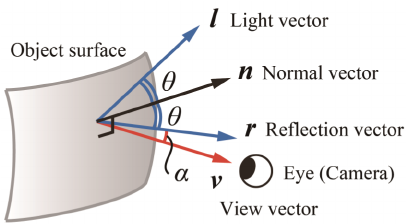
\includegraphics[width=.6\columnwidth]{figures/PhongReflectionModel.png}}
\caption{Phong reflection model \cite{kurihara2012shading}}
\label{fig:PhongReflectionModel}
\end{figure}

Digital images are generated by hardware that measures radiated energy from the source. These measurements are taken from various points across two-dimensional space to form the image. These measuring equipment are called sensors, and many different types are used. For example, sensors can interact with various parts of the electromagnetic spectrum, acoustic energy, electron emission, lasers, or other measurable signals. The electromagnetic spectrum includes visible light, infrared, ultraviolet, X-rays, microwaves, radio waves, or gamma rays (see Figure \ref{fig:EMSpectrumcolor}) [6].

\begin{figure}[htbp]
\centering
\fbox{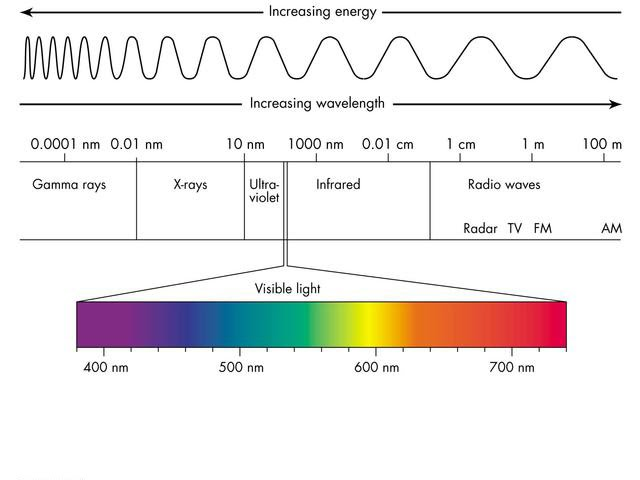
\includegraphics[width=.8\columnwidth]{figures/EMSpectrumcolor.jpg}}
\caption{Electromagnetic spectrum \cite{ElectromagneticSpectrum}}
\label{fig:EMSpectrumcolor}
\end{figure}

\subsection{BINARY, GREY-LEVEL AND COLOR IMAGES}

Binary images are the simplest form of imagery which can be typically represented as "black" and "white" or "0" and "1". A binary image assigns 1-bit to each pixel image which is enough to represent each pixel \cite{umbaugh2005computer, costa2000shape}. In addition, binary images are often produced according to a defined threshold value from gray-level images. Here, each pixel above the threshold value gets the value "1", and the one below the threshold value "0" \cite{umbaugh2005computer, costa2000shape}.

Gray-level images do not contain color information and only describe luminance information, also referred to as monochrome images. The number of bits used for each pixel is defined by the number of different brightness levels available. For example, a typical image contains 8-bits per pixel, which allows us to have 256 (0-255) different brightness (gray) levels \cite{umbaugh2005computer, costa2000shape}.

Color images are expressed using color models that contain three or more values for all pixels. Therefore, at least three two-dimensional matrices should express color images. Some of the most popular color display systems are RGB (Red, Green, Blue), CMY (greenish blue, magenta, yellow), and HIS (hue, vibrancy, intensity) \cite{costa2000shape}. If the 8-bit monochrome image is used as the standard model, the corresponding color image should be 24-bit, with 8 bits for all color bands (Red, green, blue) for each pixel \cite{umbaugh2005computer}.

\subsection{IMAGE PROCESSING AND FILTERING}

Image Processing can be used to remove noise from an image with a process that we can classify as image filtering. If an image has one or more noise, it should be filtered using appropriate techniques. Improved images with less noise can be obtained with special filter applications \cite{costa2000shape}

Local processing is often required for the analysis of image screens. Since the character structure of the image to be processed can vary significantly from one region to another, it is natural that local processing is necessary. Many image processes can produce output information depending on the neighbors of the pixels of the image given as input information. In reality, there are many approaches based on this idea, often using sliding windows and varying from convolution to mathematical structure \cite{costa2000shape}.

The kernel is a small matrix used in the convolutions of the image. Kernels of different sizes covering different patterns of numbers lead to different results under convolution. For example, Table \ref{tab:Kernal3_3} shows a 3x3 kernel presenting an average filter.

\begin{table}[htbp]
\begin{center}
\caption{3x3 Kernel (box blur)}
\vspace{23pt}
      \begin{tabular}{|l|l|l|}
        \hline
        1 & 1 & 1   \\
        \hline
        1 & 1 & 1   \\
        \hline
        1 & 1 & 1   \\
        \hline
      \end{tabular}
\label{tab:Kernal3_3}
\end{center}
\end{table}

Convolution is applied by shifting the kernel on the image, usually starting from the upper left corner of the image. This operation takes place in all positions where the kernel will be applied, within the borders of the whole image, by moving the kernel. This application differs on the edges of the images. Each core position corresponds to a single pixel output calculated by multiplying the kernel values with the pixel value of the image and the sum of all these numbers together \cite{russ2010image}. Mathematically expressed formula of the convolution can be seen in \ref{convolution_kernel} where  \(\xi\) is the filter kernel and \(f(x,y)\) is the image.

\begin{equation} \label{convolution_kernel}
d(x,y) = \xi * f(x,y) = \sum_{dx=-a}^{a} \sum_{dy=-b}^{b} \xi(dx,dy) f(x + dx, y + dy)
\end{equation}

Convolution can be implemented with different kernels for various purposes such as blurring or edge detection, such as the Gaussian filter and the Sobel Edge Detection Operators. A few of the popular filters will be discussed in the coming paragraphs.

The box blur which replaces each pixel value of an image with the average value, including its neighbors and itself. Therefore, this operation results in the disappearance of pixel values that are not representative of their surroundings. This type of filtering reduces the relative differences between the neighboring pixels of the image and improves contrast by reducing noise and smoothing.

The second is the Gaussian filter, a convolution operator used to remove detail and noise and blur images. Therefore, it performs similar result to the box blur, but the Gaussian operator uses a different kernel, represented as a bell \cite{getreuer2013survey} (see equation \ref{gaussian_filter})

\begin{equation} \label{gaussian_filter}
G(x) = \frac{1} { {\sigma \sqrt {2\pi } } } 
e^{
    {
        { - {x} ^2 }
        \mathord{\left/ {\vphantom {{ - \left( {x - \mu } \right)^2 } {2\sigma ^2 }}} \right. \kern-\nulldelimiterspace} {2\sigma ^2 }
    }
}
\end{equation}

The effect of the Gaussian operator is to blur the image, as in the box blur filter. The Gaussian standard deviation determines the degree of blurring. Kernels used for a Gaussian with a more significant standard deviation will have larger dimensions. It produces the output by averaging the Gaussian center in the direction of the pixels. Therefore, it performs a smoother operation relative to the box blur filter and reveals better edges than a Gaussian similar-sized the box blur filter \cite{getreuer2013survey}.

The last one is the median filter frequently used to reduce the noise in the images. As in the box blur, the median filter evaluates the pixels in the image together with the neighboring pixels. However, instead of taking the neighboring pixel values' average, it takes the neighboring pixel values' median and replaces the pixel value \cite{russ2010image}.

\subsection{EDGE DETECTION}

Edges are places in the image that have significant brightness changes. Therefore, edge detection is widely used to detect the object boundaries that usually occur in the image regions. In addition, creating the image with the edges of the image can significantly reduce the amount of data while retaining most of the image information \cite{russ2010image}.

Since the edges are mainly composed of high frequencies, the edges can be detected by applying a high-pass frequency filter in the Fourier region or by convolution the image with a kernel. However, edges are detected by applying convolution with a specific kernel in practice because it is cheaper and gives better results \cite{russ2010image}.

The edges can also be found by calculating the derivatives of the image since they correspond to substantial illuminance. Therefore the edges can be detected by the maximum of the first derivative and the zero of the second derivative.

Different edge detection kernels make it possible to calculate an image's first and second derivatives. For example, Prewitt Compass Edge Detection \cite{prewitt1970object}, and Gradient Edge Detection operators \cite{bovik2010handbook} are two common approaches for calculating the first derivative of an image. 

Prewitt Compass Edge Detection involves convolution of the image by adjusting the kernel sensitivity to identify a different edge. It determines the kernel edge size and definition that produces the maximum response at a pixel location. On the other hand, Gradient Edge Detection is a second and more widely used technique. Here, the image is convoluted with only two kernels for the x-direction and y-direction. The Sobel, Roberts Cross, and Prewitt operators are the most common kernels used as gradient edge detection detectors.

In Gradient Edge Detection, the pixels related to the edge need to be defined after calculating the magnitude of the first derivative. The simplest way is to set a threshold and consider all pixels with a local value above the threshold to display edges. An alternative technique to a gradient image is to identify one pixel-wide edge at the local maximum point, which is a more common technique used by the Canny edge detection method. Canny first applies Gradient edge detection to the image and then finds the edge pixels by cutting non-maximum points and tracking hysteresis \cite{moeslund2009image}.
